
\documentclass{standalone}
\usepackage{xcolor}
\usepackage{pgfplots}
\pgfplotsset{compat=1.18}

\begin{document}

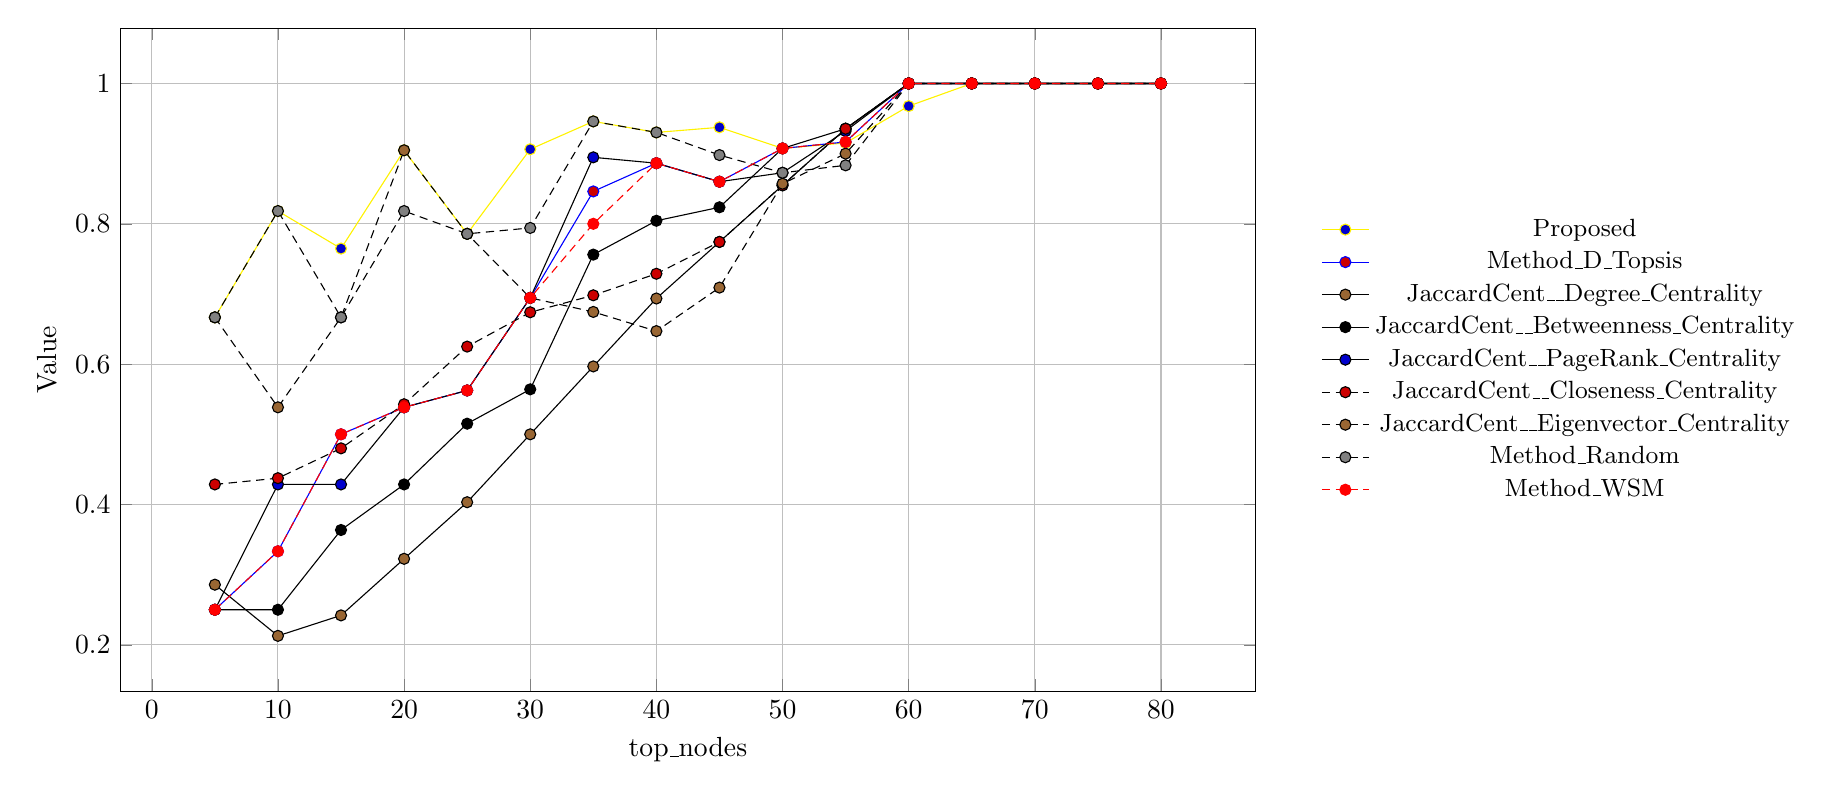
\begin{tikzpicture}
\begin{axis}[
    width=16cm,
    height=10cm,
    xlabel={top\_nodes},
    ylabel={Value},
    grid=major,
    legend style={
        at={(1.05,0.5)},
        anchor=west,
        font=\small,
        draw=none,
        cells={align=left},
    },
]
% Proposed
\addplot+[color=yellow, mark=*] coordinates {
(5.0,0.6666666666666666) (10.0,0.8181818181818182) (15.0,0.7647058823529411) (20.0,0.9047619047619048) (25.0,0.7857142857142857) (30.0,0.90625) (35.0,0.945945945945946) (40.0,0.9302325581395348) (45.0,0.9375) (50.0,0.9074074074074074) (55.0,0.9152542372881356) (60.0,0.967741935483871) (65.0,1.0) (70.0,1.0) (75.0,1.0) (80.0,1.0) };
\addlegendentry{Proposed}

% Method\_D\_Topsis
\addplot+[color=blue, mark=*] coordinates {
(5.0,0.25) (10.0,0.3333333333333333) (15.0,0.5) (20.0,0.5384615384615384) (25.0,0.5625) (30.0,0.6944444444444444) (35.0,0.8461538461538461) (40.0,0.8863636363636364) (45.0,0.86) (50.0,0.9074074074074074) (55.0,0.9166666666666666) (60.0,1.0) (65.0,1.0) (70.0,1.0) (75.0,1.0) (80.0,1.0) };
\addlegendentry{Method\_D\_Topsis}

% JaccardCent\_\_Degree\_Centrality
\addplot+[color=black, mark=*] coordinates {
(5.0,0.2857142857142857) (10.0,0.2127659574468085) (15.0,0.2419354838709677) (20.0,0.3225806451612903) (25.0,0.4032258064516129) (30.0,0.5) (35.0,0.5967741935483871) (40.0,0.6935483870967742) (45.0,0.7741935483870968) (50.0,0.8548387096774194) (55.0,0.935483870967742) (60.0,1.0) (65.0,1.0) (70.0,1.0) (75.0,1.0) (80.0,1.0) };
\addlegendentry{JaccardCent\_\_Degree\_Centrality}

% JaccardCent\_\_Betweenness\_Centrality
\addplot+[color=black, mark=*] coordinates {
(5.0,0.25) (10.0,0.25) (15.0,0.3636363636363636) (20.0,0.4285714285714285) (25.0,0.5151515151515151) (30.0,0.5641025641025641) (35.0,0.7560975609756098) (40.0,0.8043478260869565) (45.0,0.8235294117647058) (50.0,0.9074074074074074) (55.0,0.935483870967742) (60.0,1.0) (65.0,1.0) (70.0,1.0) (75.0,1.0) (80.0,1.0) };
\addlegendentry{JaccardCent\_\_Betweenness\_Centrality}

% JaccardCent\_\_PageRank\_Centrality
\addplot+[color=black, mark=*] coordinates {
(5.0,0.25) (10.0,0.4285714285714285) (15.0,0.4285714285714285) (20.0,0.5384615384615384) (25.0,0.5625) (30.0,0.6944444444444444) (35.0,0.8947368421052632) (40.0,0.8863636363636364) (45.0,0.86) (50.0,0.8727272727272727) (55.0,0.9322033898305084) (60.0,1.0) (65.0,1.0) (70.0,1.0) (75.0,1.0) (80.0,1.0) };
\addlegendentry{JaccardCent\_\_PageRank\_Centrality}

% JaccardCent\_\_Closeness\_Centrality
\addplot+[color=black, mark=*] coordinates {
(5.0,0.4285714285714285) (10.0,0.4375) (15.0,0.48) (20.0,0.5428571428571428) (25.0,0.625) (30.0,0.6739130434782609) (35.0,0.6981132075471698) (40.0,0.7288135593220338) (45.0,0.7741935483870968) (50.0,0.8548387096774194) (55.0,0.935483870967742) (60.0,1.0) (65.0,1.0) (70.0,1.0) (75.0,1.0) (80.0,1.0) };
\addlegendentry{JaccardCent\_\_Closeness\_Centrality}

% JaccardCent\_\_Eigenvector\_Centrality
\addplot+[color=black, mark=*] coordinates {
(5.0,0.6666666666666666) (10.0,0.5384615384615384) (15.0,0.6666666666666666) (20.0,0.9047619047619048) (25.0,0.7857142857142857) (30.0,0.6944444444444444) (35.0,0.6744186046511628) (40.0,0.6470588235294118) (45.0,0.7090909090909091) (50.0,0.8571428571428571) (55.0,0.9) (60.0,1.0) (65.0,1.0) (70.0,1.0) (75.0,1.0) (80.0,1.0) };
\addlegendentry{JaccardCent\_\_Eigenvector\_Centrality}

% Method\_Random
\addplot+[color=black, mark=*] coordinates {
(5.0,0.6666666666666666) (10.0,0.8181818181818182) (15.0,0.6666666666666666) (20.0,0.8181818181818182) (25.0,0.7857142857142857) (30.0,0.7941176470588235) (35.0,0.945945945945946) (40.0,0.9302325581395348) (45.0,0.8979591836734694) (50.0,0.8727272727272727) (55.0,0.8833333333333333) (60.0,1.0) (65.0,1.0) (70.0,1.0) (75.0,1.0) (80.0,1.0) };
\addlegendentry{Method\_Random}

% Method\_WSM
\addplot+[color=red, mark=*] coordinates {
(5.0,0.25) (10.0,0.3333333333333333) (15.0,0.5) (20.0,0.5384615384615384) (25.0,0.5625) (30.0,0.6944444444444444) (35.0,0.8) (40.0,0.8863636363636364) (45.0,0.86) (50.0,0.9074074074074074) (55.0,0.9166666666666666) (60.0,1.0) (65.0,1.0) (70.0,1.0) (75.0,1.0) (80.0,1.0) };
\addlegendentry{Method\_WSM}


\end{axis}
\end{tikzpicture}

\end{document}
